\documentclass[12pt]{beamer}

\usepackage[utf8]{inputenc}
\usepackage[T1]{fontenc}
\usepackage[croatian]{babel}

\usepackage{bm}
\usepackage{multirow}
\usepackage{graphicx}

\graphicspath{ {./images/} }

\newcommand{\eng}[1]{(engl. \textsl{#1}\/)}
\newcommand{\vect}[1]{\bm{\mathsf{#1}}}

\usetheme{metropolis}           % Use metropolis theme

\title{Uklanjanje šuma na slikama iscrtanim Monte Carlo
metodama primjenom dubokih konvolucijskih modela}
\date{29. siječnja 2019.}
\author{Nikola Bunjevac}
\institute{Fakultet elektrotehnike i računarstva}

\begin{document}
  \maketitle

  \begin{frame}{Sadržaj}
    \tableofcontents
  \end{frame}

  \section{Problem}

  \begin{frame}{Problem}
    \begin{itemize}
    \item Jednadžba iscrtavanja \eng{rendering equation}
    \end{itemize}
    \begin{math}
      \mathsf{L_o}(\vect{p}, \vect{\omega}_{\mathsf{o}}) = \mathsf{L_e}(\vect{p}, \vect{\omega}_{\mathsf{o}}) + \int_{\mathsf{S^2}} \mathsf{f}(\vect{p}, \vect{\omega}_{\mathsf{o}}, \vect{\omega}_{\mathsf{i}}) \mathsf{L_i}(\vect{p}, \vect{\omega}_{\mathsf{i}}) |\cos\theta_i| \mathsf{d}\vect{\omega}_{\mathsf{i}}
    \end{math}

    \begin{itemize}
    \item Monte Carlo integracija (uzorkovanje)
    \end{itemize}
    \begin{center}
    \begin{tabular}{c}
      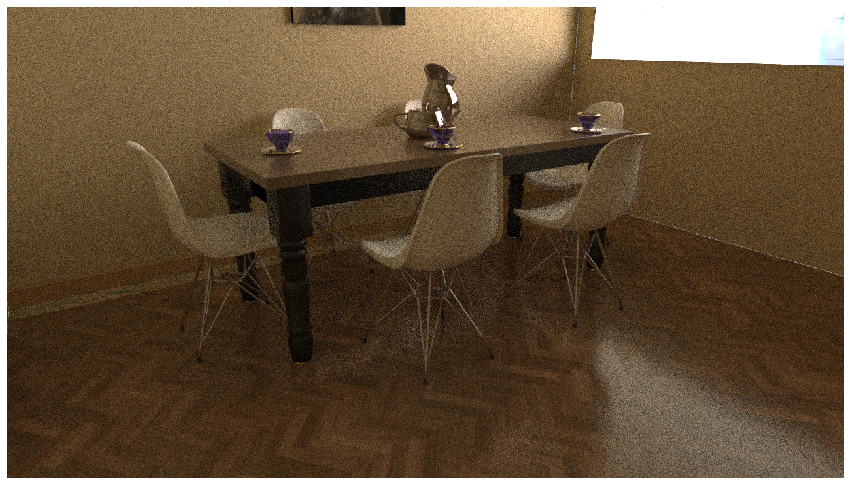
\includegraphics[width=0.65\textwidth]{noisy_color.png}
    \end{tabular}
    \end{center}
    \begin{itemize}
    \item Cilj: ukloniti šum bez dodatnih uzorkovanja
    \end{itemize}


  \end{frame}

  \begin{frame}{Dodatne značajke}
    \begin{itemize}
    \item Potrebne su nam dodatne značajke poput normala, albeda, dubine...
          \begin{itemize}
    \item Izlaz iz iscrtavatelja \eng{renderer}
    \end{itemize}
    \end{itemize}
    \begin{center}
      \makebox[\linewidth]{
    \begin{tabular}{ccc}
            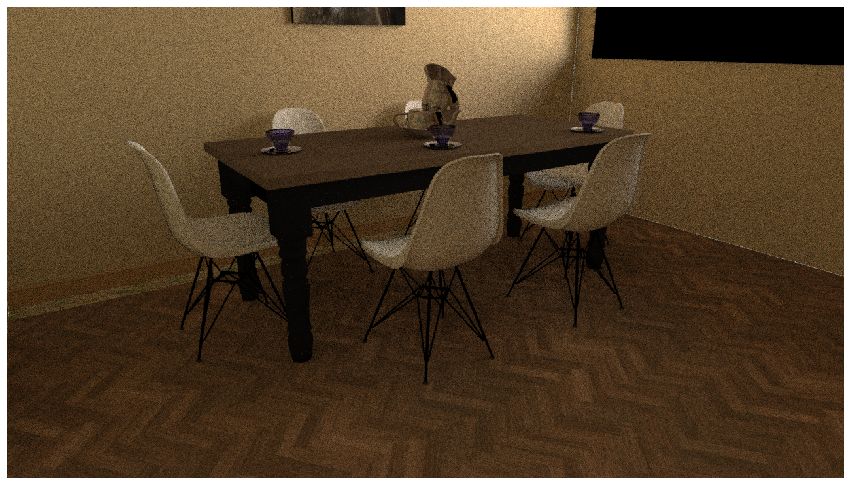
\includegraphics[width=0.33\textwidth]{noisy_diffuse.png} &   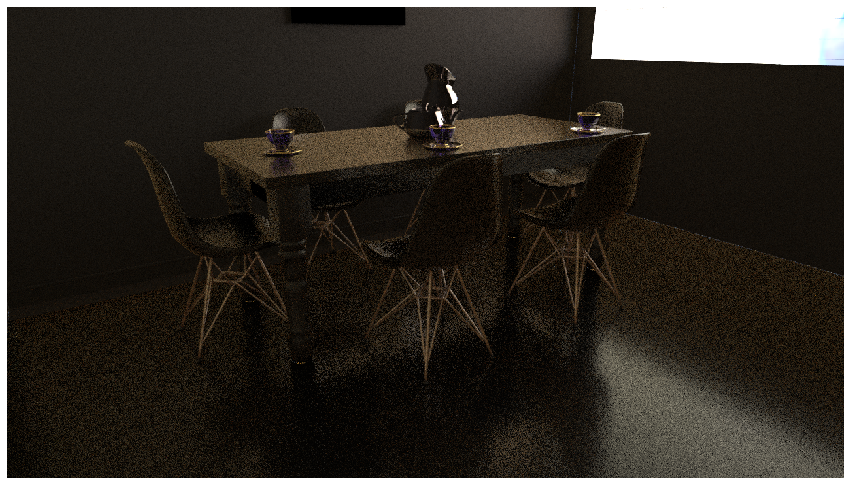
\includegraphics[width=0.33\textwidth]{noisy_specular.png} & 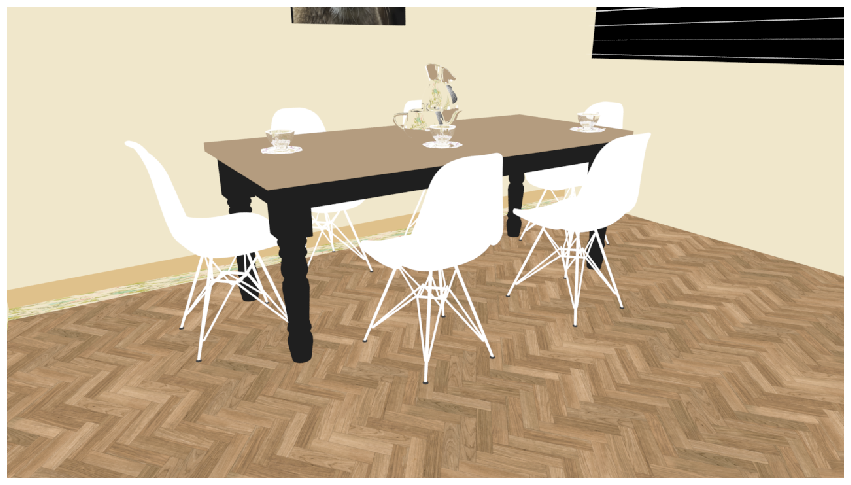
\includegraphics[width=0.33\textwidth]{noisy_albedo.png} \\
        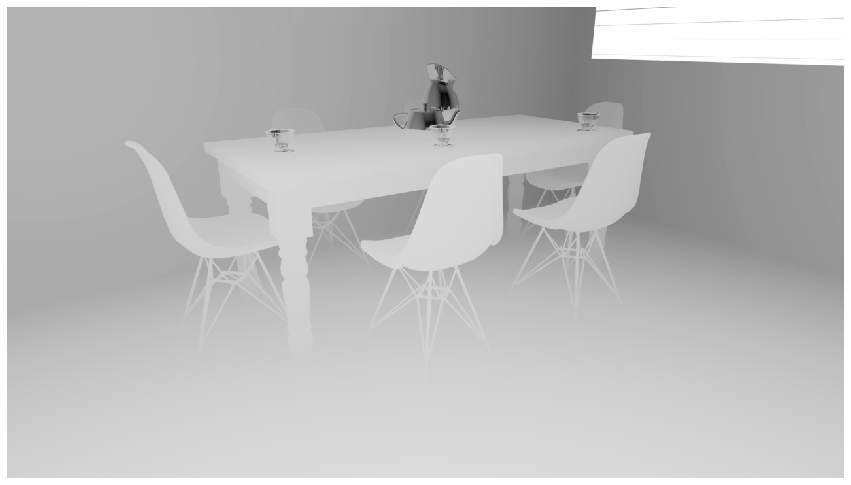
\includegraphics[width=0.33\textwidth]{noisy_depth.png} & 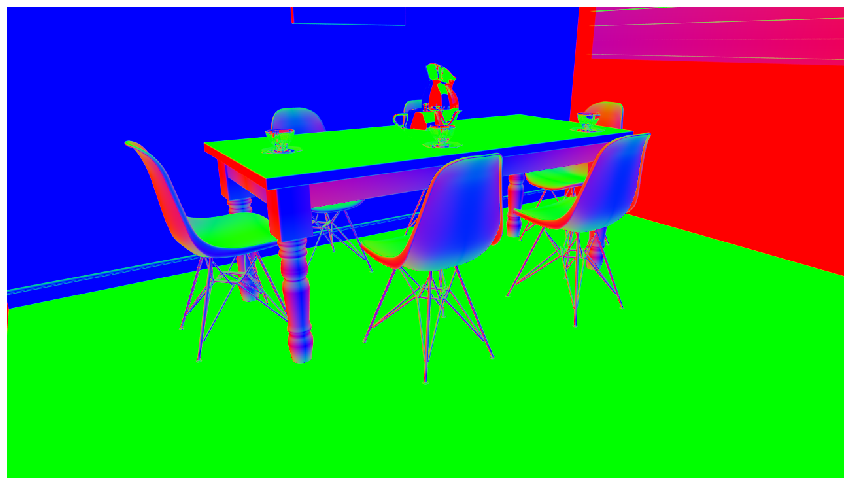
\includegraphics[width=0.33\textwidth]{noisy_normals.png} &   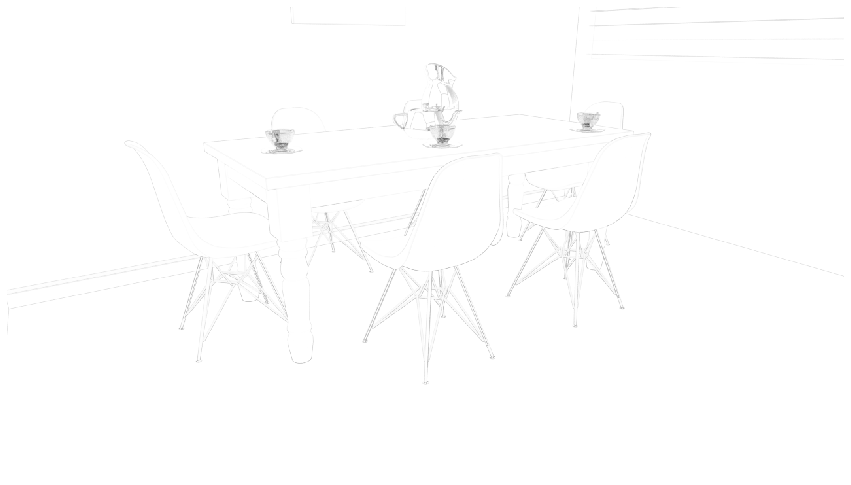
\includegraphics[width=0.33\textwidth]{noisy_normalVariance.png} \\
    \end{tabular}}
    \end{center}

  \end{frame}

  \section{Model}
  \begin{frame}{Model}
    \begin{itemize}
    \item Duboki konvolucijski model
      \begin{itemize}
        \item Dvije podmreže - difuzna i zrcalna
      \item 9 slojeva, 100 jezgri $5 \times 5$, ReLU (osim na izlazu)
      \end{itemize}
      \item Dvije varijante modela (razlika u zadnjem sloju)
    \begin{enumerate}
    \item Izravna predikcija
    \item Predikcija pomoću jezgre
    \end{enumerate}
    \end{itemize}

    \begin{center}
    \begin{tabular}{c}
      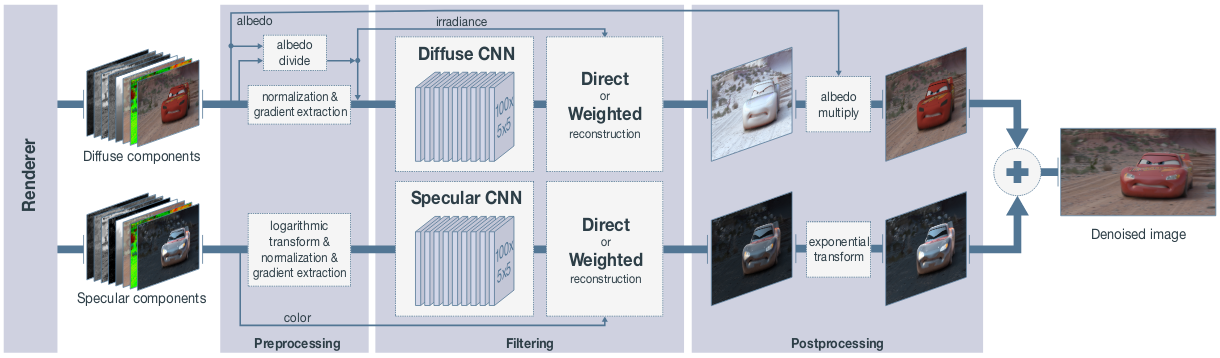
\includegraphics[width=\textwidth]{architecture.png}
    \end{tabular}
    \end{center}
  \end{frame}

  \section{Rezultati}

  \begin{frame}{Vrijeme učenja}
    \begin{itemize}
    \item Obje varijante mogu doći do iste pogreške, ali predikcija pomoću jezgre brže
    \end{itemize}

    \begin{center}
      \makebox[\linewidth]{
      \begin{tabular}{cc}
        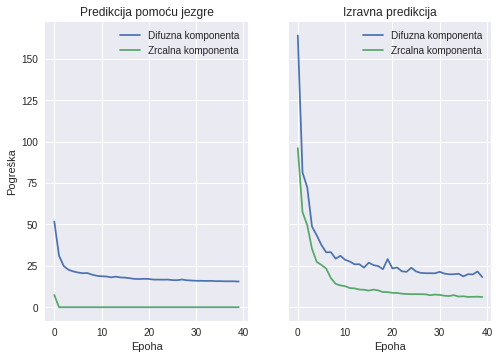
\includegraphics[width=0.5\textwidth]{time_my.png} & 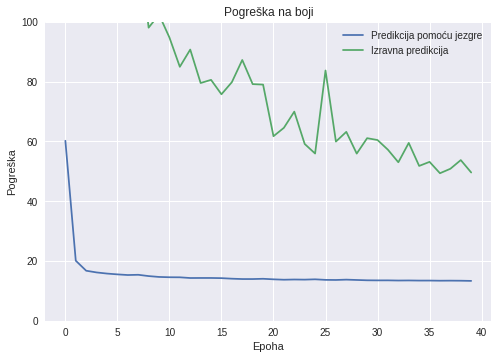
\includegraphics[width=0.5\textwidth]{model_time.png}
      \end{tabular}
      }
    \end{center}
  \end{frame}

  \begin{frame}{Primjer uklanjanja šuma}
    \begin{center}
      \makebox[\linewidth]{
        \begin{tabular}{ccc}
          \multirow{2}{*}{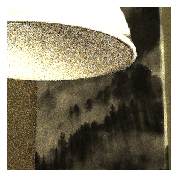
\includegraphics[width=0.3\textwidth]{eval1_in.png}}
        & 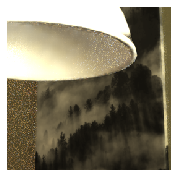
\includegraphics[width=0.3\textwidth]{eval1_kpcn.png} &
          \multirow{2}{*}{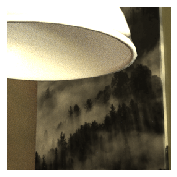
\includegraphics[width=0.3\textwidth]{eval1_ref.png}} \\
          & 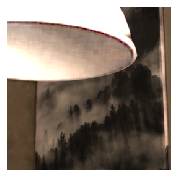
\includegraphics[width=0.3\textwidth]{eval1_dpcn.png} & \\
      \end{tabular}}
      \end{center}
  \end{frame}

    \begin{frame}{Primjer uklanjanja šuma}
      \begin{center}
        \makebox[\linewidth]{
          \begin{tabular}{c}
            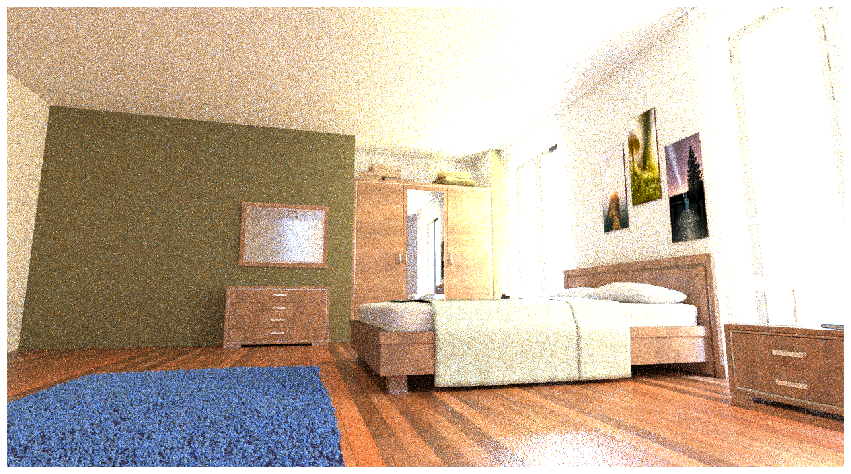
\includegraphics[width=\textwidth]{eval4_in.png}
        \end{tabular}}
      \end{center}
    \end{frame}

        \begin{frame}{Primjer uklanjanja šuma}
      \begin{center}
        \makebox[\linewidth]{
          \begin{tabular}{c}
            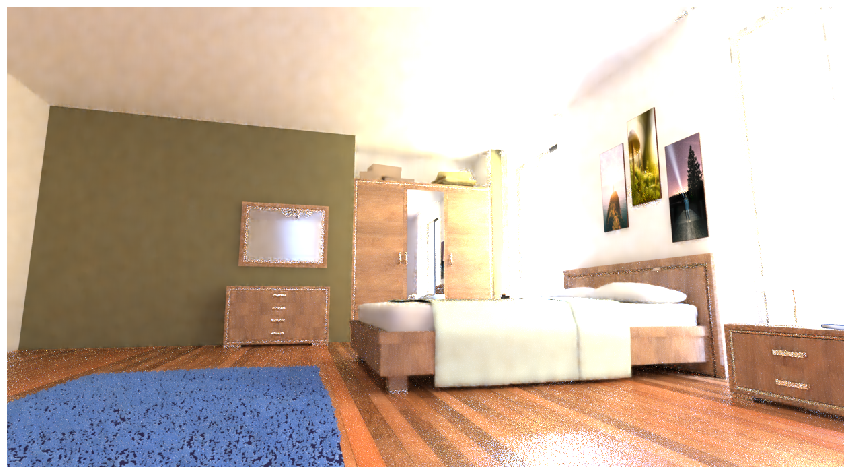
\includegraphics[width=\textwidth]{eval4_kpcn.png}
        \end{tabular}}
      \end{center}
        \end{frame}

                \begin{frame}{Primjer uklanjanja šuma}
      \begin{center}
        \makebox[\linewidth]{
          \begin{tabular}{c}
            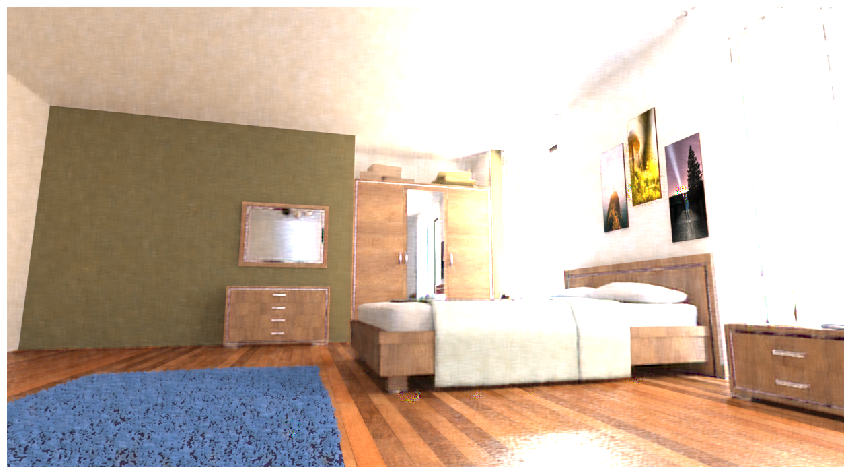
\includegraphics[width=\textwidth]{eval4_dpcn.png}
        \end{tabular}}
      \end{center}
    \end{frame}

  \section{Zaključak}

  \begin{frame}{Zaključak}
    \begin{itemize}
    \item Jednostavan, ali učinkovit model
    \item Ima prostora za napredak
    \item Temporalna nestabilnost
    \item Korištenje u stvarnom vremenu
    \end{itemize}
  \end{frame}

\end{document}
